% Harry's website evaluation 
\section{Harry's Evaluation}
\subsection{Scores}
Outlined below are the evaluations provided by Harry Foley for the Nielsen and MILE heuristics carefully selected by the group to analyze the website.\\
% Nielsen's Heuristics Evaluation
\begin{table}[htp!]
    \centering
    \begin{tabular}{ |l|l|c| }
        \hline
        \textbf{Code} & \textbf{Description} & \textbf{Score}\\
        \hline
        \textbf{H1} & Visibility of system status & \textbf{\color{unicefRed}{2}}\\
        \hline
        \textbf{H2} & Match between system and the real world & \textbf{\color{unicefGreen}{5}}\\
        \hline
        \textbf{H3} & User control and freedom & \textbf{\color{unicefRed}{3}}\\
        \hline
        \textbf{H4} & Consistency and standards & \textbf{\color{unicefGreen}{5}}\\
        \hline
        \textbf{H5} & Error prevention & \textbf{\color{unicefGreen}{5}}\\
        \hline
        \textbf{H6} & Recognition rather than recall & \textbf{\color{unicefGreen}{4}}\\
        \hline
        \textbf{H7} & Flexibility and efficiency of use & \textbf{\color{unicefRed}{2}}\\
        \hline
        \textbf{H8} & Aesthetic and minimalist design & \textbf{\color{unicefGreen}{4}}\\
        \hline
        \textbf{H9} & Help users recognize, diagnose and recover from errors & \textbf{\color{unicefGreen}{5}}\\
        \hline
        \textbf{H10} & Help and documentation & \textbf{\color{unicefGray}{n.a}}\\
        \hline
    \end{tabular}
    \caption{\textbf{Nielsen}'s heuristics scores}
\end{table}
% MILE Heuristics Evaluation
\begin{table}[htp!]
    \centering
    \begin{tabular}{ |c|l|l|c| }
        \hline
        \textbf{Group} & \textbf{Code} & \textbf{Description} & \textbf{Score}\\
        \hline
        \multirow{5}{*}{\textbf{Navigation}} & \textbf{M1} & Interaction consistency & \textbf{\color{unicefGreen}{4}}\\
        \cline{2-4}
        & \textbf{M2} & Group navigation & \textbf{\color{unicefRed}{2}}\\
        \cline{2-4}
        & \textbf{M3} & Navigation support & \textbf{\color{unicefRed}{2}}\\
        \cline{2-4}
        & \textbf{M4} & User control & \textbf{\color{unicefRed}{1}}\\
        \cline{2-4}
        & \textbf{M5} & Error prevention & \textbf{\color{unicefOrange}{3}}\\
        \hline
        \textbf{Content} & \textbf{M6} & Information overload & \textbf{\color{unicefOrange}{3}}\\
        \hline
        \multirow{6}{*}{\textbf{Presentation}} & \textbf{M7} & Text layout & \textbf{\color{unicefGreen}{5}}\\
        \cline{2-4}
        & \textbf{M8} & Interaction placeholder semiotics & \textbf{\color{unicefGreen}{5}}\\
        \cline{2-4}
        & \textbf{M9} & Interaction placeholder consistency & \textbf{\color{unicefGreen}{5}}\\
        \cline{2-4}
        & \textbf{M10} & Spatial allocation & \textbf{\color{unicefGreen}{4}}\\
        \cline{2-4}
        & \textbf{M11} & Consistency of the page structure & \textbf{\color{unicefGreen}{4}}\\
        \cline{2-4}
        & \textbf{M12} & Coherence in page layout & \textbf{\color{unicefGreen}{5}}\\
        \hline
    \end{tabular}
    \caption{\textbf{MILE} heuristics scores}
\end{table}
% Comments 
\newpage
\subsection{Comments}
This section offers clear and concise explanations and justifications for the scores assigned to the previously presented heuristics.
% Nielsen's Heuristics Comments
\subsubsection{Nielsen's Heuristics}
\begin{description}
    \item {\textbf{H1} \color{unicefGray}{Visibility of the system status}}\\
    breadcrumbs and user paths are only provided in some areas of the website. For example, If a user is exploring pages in the “What We Do” section strong bread crumbs are provided, that are clear and useful. 
    However other areas of the site such as “Research and Reports” do not provide any bread crumbs.
    \item {\textbf{H2} \color{unicefGray}{Match between system and the real world}}\\
    Language used on the site is clear and simple. Symbols used throughout the site are logical and uncomplicated.     
    \newpage
    \item {\textbf{H3} \color{unicefGray}{User control and freedom}}\\
    Only applicable where bread crumb paths are provided. Allows the user to easily navigate backwards or move to other relevant subsections. 
    One issue is that at some stages of exploring the website clicking the unicef button at the top left of the page will only bring you back to the home of that section of the website. 
    For example when in “unicef.org/ethics/” users cannot get back to "unicef.org" without editing the website address manually.
    When making a donation it is possible for the user to “undo” or go back to the previous step without restarting the process, and the system remembers the user’s inputted data. 
    \begin{figure}[h]
        \centering
        
\includegraphics[scale=1.0]{Resources/Harry/Harry_H3.png}
        \caption{User forced to edit URL to return to unicef.org}
    \end{figure}
    \item {\textbf{H4} \color{unicefGray}{Consistency and standards}}\\
	I did not find any errors in consistency or standards.    
    \item {\textbf{H5} \color{unicefGray}{Error prevention}}\\
    Standard error prevention implemented such as only allowing number characters to be inserted in phone number fields, or checking email address matches the correct formatting. 
    \begin{figure}[h]
        \centering
        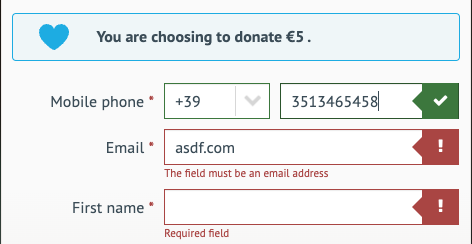
\includegraphics[scale=1.0]{Resources/Harry/Harry_H5.png}
        \caption{Error prevention in the donation section}
    \end{figure}
    \item {\textbf{H6} \color{unicefGray}{Recognition rather than recall}}\\
    The search function provides auto suggestions to reduce user’s memory load. When making a donation the user is reminded at each step of the process how much their donation will be. 
    \item {\textbf{H7} \color{unicefGray}{Flexibility and efficiency of use}}\\
    The website does not provide the ability for users to be able to tailor frequent actions. No accelerators are provided either. The only way an advanced user can use the site more efficiently is by learning where certain information is or knowing what to specifically search. 
    \item {\textbf{H8} \color{unicefGray}{Aesthetic and minimalist design}}\\
    The website has a consistent minimal design throughout. The site has quite a basic aesthetic using primarily blue and grey colours. Some minimal shadowing is added to various cards and banners to give a depth effect. The only places that red is used is for donations, this helps to bring the user’s eye to it. 
    \newpage
    \begin{figure}[h]
        \centering
        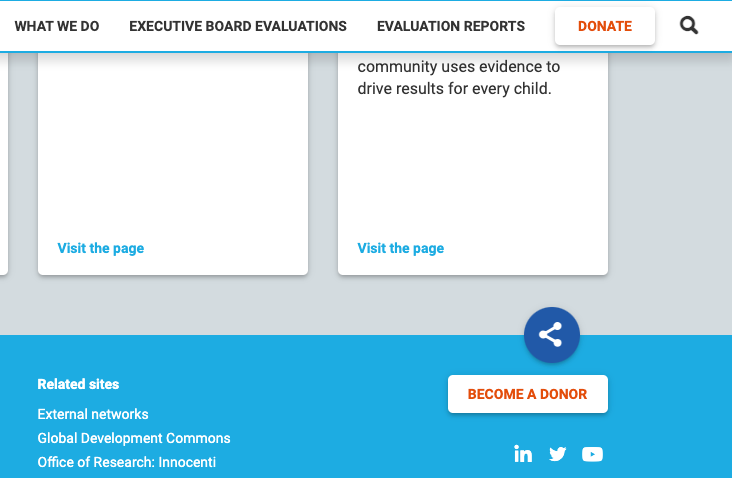
\includegraphics[scale=1.0]{Resources/Harry/Harry_H8.png}
        \caption{Example of the website's use of colour}
    \end{figure}
    \item {\textbf{H9} \color{unicefGray}{Help users recognize, diagnose and recover from errors}}\\
    Help is provided when a user makes an error at the various stages of the donation process. The help is clear and uncomplicated.
    \begin{figure}[h]
        \centering
        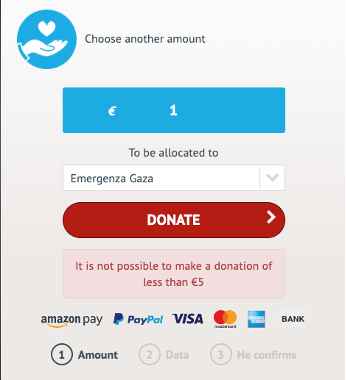
\includegraphics[scale=1.0]{Resources/Harry/Harry_H9.png}
        \caption{Help is provided when the user tries to enter an invalid donation amount}
    \end{figure}
    \item {\textbf{H10} \color{unicefGray}{Help and documentation}}\\
    Not applicable.
\end{description}
% MILE Heuristics Comments
\newpage
\subsubsection{MILE Heuristics}
\begin{description}
    \item {\textbf{M1} \color{unicefGray}{Interaction consistency}}\\
    I found that interaction consistency is strong enough throughout the site that it does not impact the user’s experience. 
    \item {\textbf{M2} \color{unicefGray}{Group navigation}}\\
    Not consistent throughout the website. When bread crumb paths are provided it is easy to navigate, without them however the site can be confusing. 
    \item {\textbf{M3} \color{unicefGray}{Structural Navigation}}\\
    I felt that it was not consistent throughout the site. 
    \item {\textbf{M4} \color{unicefGray}{Semantic Navigation}}\\
    •	Again the site is not very consistent in navigation. Primary issue with this is that the “home” feature does not always bring the user back to the main homepage of the site but instead the homepage of a topic. User can only get to the main home page then by editing the URL
    \item {\textbf{M5} \color{unicefGray}{landmarks}}\\
    The home button issue is a negative here. Apart from that, the landmarks are useful.
    \item {\textbf{M6} \color{unicefGray}{Information overload}}\\
    Although information is well laid out on each page, there is still an overwhelming amount of information per page. 
    \item {\textbf{M7} \color{unicefGray}{Text layout}}\\
    Text is off an appropriate size and readable throughout the site.
    \item {\textbf{M8} \color{unicefGray}{Interaction placeholder semiotics}}\\
    Yes, semiotics are intuitive and convey their functional meaning. I did not feel any ambiguity when using the interactive elements.
    \begin{figure}[h]
        \centering
        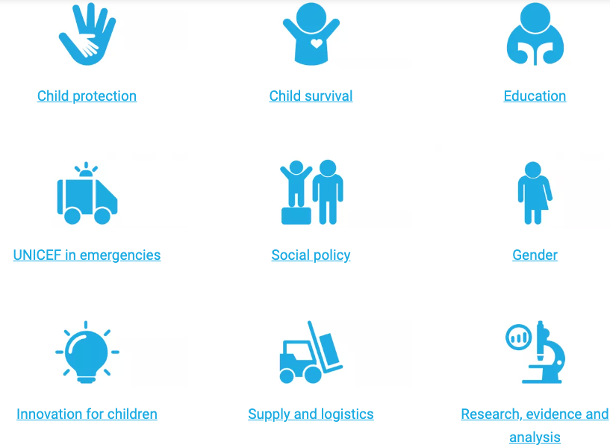
\includegraphics[scale=1.0]{Resources/Harry/Harry_M8.png}
        \caption{Example of the semiotics used in the website}
    \end{figure}
    \item {\textbf{M9} \color{unicefGray}{Interaction placeholder consistency}}\\
    Yes, the interaction placeholders feel consistent throughout the site. 
    \item {\textbf{M10} \color{unicefGray}{Spatial allocation}}\\
    Not applicable on every page. Where it does occur it is sufficient for the user to understand that items/elements belong together due to their type.
    \begin{figure}[h]
        \centering
        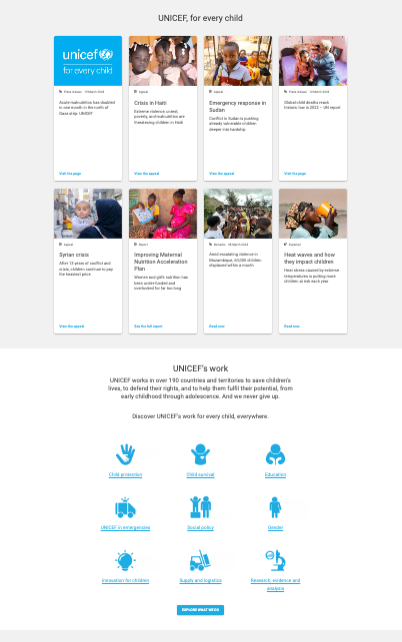
\includegraphics[scale=1.0]{Resources/Harry/Harry_M10.png}
        \caption{An example of the websites use of space to group items}
    \end{figure}
    \item {\textbf{M11} \color{unicefGray}{Consistency of the page structure}}\\
    Yes, pages of the same type have a consistent structure. These types of pages are easily identified by including a label like “Article” or “Blog Post”.
    \item {\textbf{M12} \color{unicefGray}{Coherence in page layout}}\\
    The website's layout is coherent and consistent, with a clear and logical structure.
\end{description}


